\chapter{Homology}
Before go into what \textit{persistent} homology it is well worth our time to clearly state what we mean by homology. Broadly speaking, homology is an invariant of topological spaces which is concerned with cycles in the space which are not boundaries. Or more abstractly, homology captures the notion $n$-dimensional holes in the space. In \textit{persistent} homology we generally work without predefined topological spaces and start with a basic data-set which at most contains some metric structure. Therefore the classical definitions involving singular homology are not something we will dwell on, but rather we refer the reader to Hatcher's excellent exposition in \cite{hatcher2002}.

The main concept we will be working with is simplicial homology since computationally we can approximate a simplicial complex on our topological spaces. This way we can compute the homological invariants without any a priori information about what topological space we are working in.

\section{Simplices}
We start with what will constitute our atoms in simplicial homology, namely the simplices.
\begin{definition}
An \textbf{$n$-simplex} is the smallest possible convex set in $\mathbb{R}^{m}$ containing $n+1$ points $v_{0},\dots,v_{n}$ such that the vectors $v_{1}-v_{0}, \dots, v_{n} - v_{0}$ are linearily independent. The points $v_{0},\dots,v_{n}$ are known as the \textbf{vertices} of the simplex.
\end{definition}
\begin{definition}
The \textbf{standard $n$-simplex} is the $n$-simplex with vertices being the unit vectors along coordinate axes
\[ \Delta^{n} := \{ (t_{0}, \dots, t_{n}) \in R^{n+1} \mid \sum_{i} t_{i} = 1, t_{i} \geq 0 \quad \forall i \}
\]
\end{definition}
As seen in Figure \ref{simplices} the $0,1,2$ and $3$-dimensional simplices are familiar shapes consisting of vertices, edges, triangles and tetrahedrons.

\begin{figure}
  \centering
  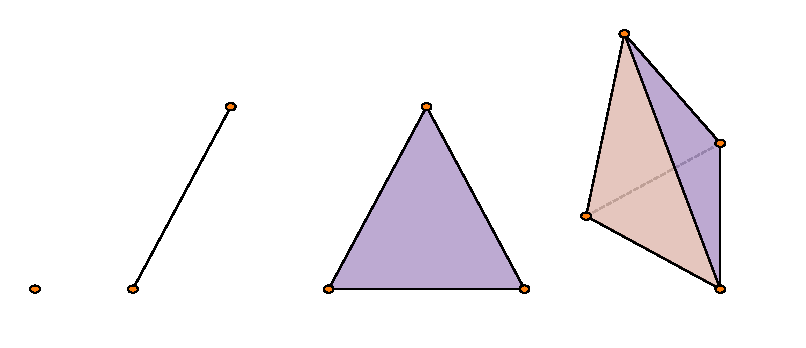
\includegraphics[]{simplex.pdf}
  \caption{
  \label{simplices}
0-simplex (left), 1-simplex (middle left), 2-simplex (middle right) and 3-simplex (right).}
  \end{figure}
\begin{definition}
A \textbf{face} of a simplex is the convex hull of a subset of its vertices.
\end{definition}
Since higher dimensional simplices are made up of simplices of lower dimensions we can always decompose a simplex into its faces, in other words the lower dimensional simplices that make up the simplex. For example, a 2-simplex can be decomposed into the three edges that make up the triangle.
\section{Simplicial complex}
By gluing together simplices at their faces as seen in Figure \ref{complex} we can construct higher-order objects which we call simplicial complexes.
\begin{definition}
A \textbf{simplicial complex} $K$ is a finite collection of simplices such that

\begin{enumerate}
    \item $\sigma \in K$ and $\tau \subset \sigma$ implies that $\tau \in K$
    \item $\sigma_{1}, \sigma_{2} \in K$ implies that $\sigma_{1} \cap \sigma_{2}$ is either empty or a face of both.
\end{enumerate}

\end{definition}
This is a geometric definition of a simplicial complex. However, since we are working with topological spaces it is advantageous to think of an abstract simplicial complex without concerning ourselves with the geometric connotations. It is possible to define a simplicial complex by only considering the ordering of the vertices and what higher-dimensional simplices they make up:

\begin{figure}
  \centering
  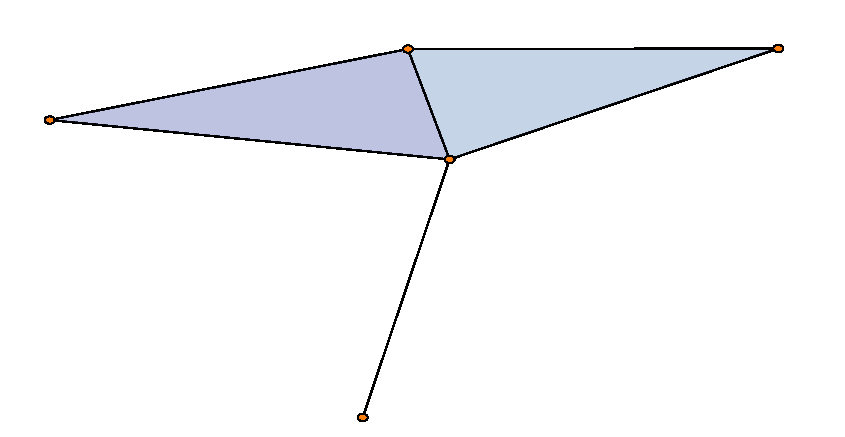
\includegraphics[scale=0.7]{complex.pdf}
  \label{complex}
  \caption{Example of a simplicial complex consisting of two 2-simplices glued together with an attached 1-simplex.}
\end{figure}

\begin{definition}[book]
An \textbf{abstract simplicial} complex $A$ is a finite collection of sets such that $\alpha \in A$ and $\beta \subseteq \alpha$ implies that $\beta \in A$.
\end{definition}

\begin{definition}[book]
An (finite) abstract simplicial complex $K$ is a collection of (finite) sets such that $\alpha \in K$ and $\beta \subseteq \alpha$ implies that $\beta \in A$.
\end{definition}

This abstract definition coincides with the geometric definition by calling the elements of $K$ its simplices. The simplices of $K$ are no longer geometric objects in Euclidean space, but simply combinatorial objects consisting of vertex sets.


% It is easy to see how one can go from a geometric simplicial complex to an abstract simplicial complex simply by forgetting everything but the vertices themselves. However, most of the time our interest lies in the opposite direction: how do we go from an abstract simplicial complex to a geometric one? This is done by the geoemtric realization of $A$.

Furthermore, we need an ordering on the simplicial complex.

\begin{definition}
An \textbf{ordered abstract simplicial complex} is an abstract simplicial complex together with a partial order ($\geq$) which restricts to a total order on each simplex.
\end{definition}


% \begin{theorem}
% Every abstract simplicial complex of dimension $d$ has a geometric realization in $\mathbb{R}^{2d+1}$.
% \end{theorem}
% \begin{proof}
% See ?.
% \end{proof}%
From here on we will simply refer to an ordered abstract simplicial complex as a simplicial complex unless stated otherwise.
\section{Simplicial homology}
Homology can generally thought of as being the characterization of cycles which are not boundaries. In the context of simplicial complexes we first need some machinery in order to define exactly what cycles and boundaries are.

\begin{definition}[\cite{Zomorodian2005}]
  The $k$th \textbf{chain module} $C_{k}(K)$ on a simplicial complex $K$ is the free module with basis given by the $k$-dimensional simplices in $K$ with coefficients in some ring $\mathcal{R}$ with additive unit $0$ and multiplicative unit $1$. In other words, the elements of $C_{k}(K)$ are formal sums
  \[ \sum_{i=1} r_{i}\sigma_{i}\]
  where $r_{i} \in \mathcal{R}$ and $\sigma_{i}$ is a $k$-dimensional simplex in $K$.
\end{definition}
\begin{definition}[{\cite[p. ~2]{weibel1994}}]
  A \textbf{chain complex} over a ring $R$ is a family of $R$-modules $\{C_{k}\}_{k
  \in \mathbb{Z}}$ with $R$-module maps $\partial_{k}: C_{i} \to C_{k-1}$ such that the composition $\partial_{k-1} \circ \partial_{k}$ is the zero map. We call the maps $\partial_{k}$ the \textbf{differentials} of the chain complex.
\end{definition}
\begin{theorem}
Given a simplicial complex $K$ and a ring $\mathcal{R}$ the sequence of chain modules
\begin{center}
\begin{tikzcd}
  \dots \arrow[]{r}{\partial_{k+1}} & C_k(K) \arrow[]{r}{\partial_{k}} & C_{k-1}(K) \arrow[]{r}{\partial_{k-1}} & C_{k-2}(K) \arrow[]{r}{\partial_{k-2}} & \dots \arrow[]{r}{\partial_{1}} & C_0(K)
\end{tikzcd}
\end{center}
with differentials defined as
\begin{align*}
& \partial_{k}:  C_{k}(K) \to C_{k-1}(K) \\
& \partial_{k}(\sigma) =  \sum^{k}_{{i=0}} (-1)^{i} [v_{0},\dots,\hat v_{i}, \dots, v_{k}]
\end{align*}
is a chain complex.
\end{theorem}

\begin{proof}
It suffices to show that $\partial_{k-1} \circ \partial_{k}$ is the zero map. (Proof missing, TODO)
  \end{proof}

% New attempt.
% For a simplicial complex $K$ of dimension we define a sequence of free abelian groups $(C_{k})$ on the (oriented?) simplices of $K$.
% The elements of $C_{k}$ are called $k$-chains and are formal sums of the type
% $\sum \alpha_{i} \sigma_{i}$
% where $\alpha_{i}$ are coefficients in some ring $R$ and $\sigma_{i}$ are $k$-dimensional simplices.
%
% Furthermore, we have a collection of homomorphisms, known as boundary maps, which together with the groups form a chain complex. The $k$th boundary map
% \[ \partial_{k}: C_{k} \to C_{k-1}\]
% takes a $k$-simplex to its boundary
% \[ \partial_{k} \sigma = \sum^{k}_{{i=0}} (-1)^{i} [v_{0},\dots,\hat v_{i}, \dots, v_{k}]\]
% where $\hat v_{i}$ signifies that this vertex has been omitted. This is a homomorphism so
% \[\partial_{k} \sum \alpha_{i}\sigma_{i} = \sum \alpha_{i} \partial_{k} \sigma_{i}\]
%
% Now a simplicial chain complex is a collection of chain groups together with their corresponding boundary maps as a sequence:
% \begin{center}
% \begin{tikzcd}
%   \dots \arrow[]{r}{\partial_{k+1}} & C_k \arrow[]{r}{\partial_{k}} & C_{k-1} \arrow[]{r}{\partial_{k-1}} & C_{k-2} \arrow[]{r}{\partial_{k-2}} & \dots
% \end{tikzcd}
% \end{center}
% Note that the boundary maps compose to become the zero map.
% \begin{theorem}
% The composed boundary map $\partial_{k+1} \circ \partial_{k}$ is the zero map.
% \end{theorem}
% \begin{proof}
% (Proof is in Hatcher. Maybe write it down, it's short and shows how boundary maps work.)
% \end{proof}
\begin{example}
Given a simplicial complex $K$ consisting of a triangle without interior as in Figure \ref{trichain}, a chain in $C_{1}(K)$ would be a linear combination of edges. For example, an element of $C_{1}(K)$ is $[v_{0},v_{1}]+[v_{1},v_{2}]$ which is highlighted in green.
\begin{figure}[ht]
  \centering
  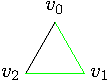
\includegraphics[scale=2]{trichain.pdf}
  \caption{\label{trichain} A simplicial complex in which the 1-chain $[v_{0},v_{1}]+[v_{1},v_{2}]$ is highlighted in green.}
\end{figure}
\end{example}

\begin{example}
Given a $2$-simplex as in Figure \ref{2simplex} we get the differential of the interior of the simplex as \[\partial_{2}([v_{0},v_{1},v_{2}])=[v_{1},v_{2}]-[v_{0},v_{2}]+[v_{1},v_{2}]\] which is the boundary of the simplex. For this reason we refer to the differential of a chain complex of a simplicial complex as the \textbf{boundary map} or \textbf{boundary operator}.
\begin{figure}[ht]
  \centering
  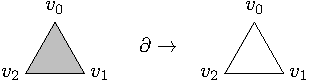
\includegraphics[scale=2]{partialtri.pdf}
  \caption{\label{2simplex} }
\end{figure}
\end{example}
We are now ready to state the definitions of cycles and boundaries.
\begin{definition}[{\cite[p. ~4]{weibel1994}}]
  Given a chain complex $C_{*}$ the \textbf{$k$-cycles} $Z_{k}$  and the \textbf{$k$-boundaries} $B_{k}$ of $K$ are the $\mathcal{R}$-modules
  \[ Z_{k} := \ker \partial_{k}\]
  \[ B_{k} := \textrm{im } \partial_{k+1}\]
\end{definition}
As mentioned our purpose of constructing this simplicial chain complex is to identify cycles which are not boundaries of higher dimensional simplices. Hence, a vital result is this corollary of (cite thm above).

\begin{corollary}
  The $k$-boundaries are a submodule of the $k$-cycles.
\end{corollary}


\begin{proof}
Let $\sigma \in B_{k} = \textrm{im } \partial_{k+1}$ then for some $\tau \in C_{k+1}$ we have that $\partial_{k+1}(\tau)=\sigma$. Hence,
\[ \partial_{k}(\sigma) = \partial_{k} \partial_{k+1}(\tau) = (\partial_{k} \circ \partial_{k+1}) \tau = 0\]
and so $\sigma \in \ker \partial_{k} = Z_{k}$.
\end{proof}
% This means that if we find a cycle in $C_{k}$ which is not in the image of $\partial_{k+1}$ then it is exactly what we are looking for. Furthermore, the boundary map of a cycle is always 0. From here comes the definition of the homology group (while we do name this the homology group to not cause confusion, it is actually a  R-module).

This tells us that there are cycles which are not boundaries and cycles which are. This motivates the following definition of homology.
\begin{definition}
  Given a simplicial chain complex \hspace{0.05cm}$C_{*}$ the homology group $H_{k}$ is defined as
  \[H_{k}(K) := Ker(\partial_{k})/Im(\partial_{k+1})\]
\end{definition}

Hence, the $k$th homology group captures precisely those cycles which are not in the image of the higher dimensional differential. In other words, the non-trivial elements are the cycles which are not boundaries.
% From this definition we know that from every simplicial complex $K$ we can associate a simplicial chain complex (this is a functor). We then define the $k$th homology group of $K$ as the quotient group
% \[H_{k}(K) = Ker(\partial_{k})/Im(\partial_{k+1})\]

% This is also a functor, so any simplicial map $K_{1} \to K_{2}$ induces a map on homology $H_{*}(K_{1}) \to H_{*}(K_{2})$.
%
\begin{example}
Figure \ref{trihom} of square + triangle, with triangle filled in.
\begin{figure}[ht]
  \centering
  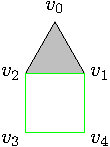
\includegraphics[scale=2]{trisquarefilled.pdf}
  \caption{\label{trihom} }
\end{figure}
Let us compute the homology of this simplicial complex consisting of a 2-simplex glued together with a square made of 1 simplices.

There are two 1-cycles, the boundary of the filled triangle and the square. Since the boundary of the filled triangle is in $Im (\partial_{2})$ we get that this element belongs to the trivial class in $H_{1}$. But there is one non-trivial element given by the square without interior. So $H_{1}$ contains one non-trivial element generated by the cycle in green.

\begin{definition}
The $k$th Betti number is the rank of the module $H_{k}$.
\end{definition}
\end{example}

%%% Local Variables:
%%% mode: latex
%%% TeX-master: "thesis.tex"
%%% End:
